
    
    \begin{tikzpicture}
        % Draw a line for the base
        \draw[thick] (0,0) -- (5,0);
        \draw[thick] (0,-0.2) -- (5,-0.2);
        \draw[thick] (0,0) -- (0,-0.2);
        \draw[thick] (5,0) -- (5,-0.2);
        \draw[thick] (0,-0.2) -- (-0.2,-0.4) -- (0.2,-0.4) -- (0,-0.2);
         \draw[thick] (5,-0.2) -- (4.8,-0.4) -- (5.2,-0.4) -- (5,-0.2);
        
        

        % Draw a force arrow
        \draw[<-, line width=0.5mm] (2.5, 0) -- (2.5, 1.5) node[above] {$200 \, \text{N}$};
            \draw[<-] (2,0) arc[start angle=179, end angle=0, radius=0.5] ;
            
    \fill (5,-0.45) circle (2pt); % 1pt radius
    \fill (4.8,-0.45) circle (2pt); % 1pt radius
    \fill (5.2,-0.45) circle (2pt); % 1pt radius

    \fill[pattern=north east lines] (-0.2,-0.4) rectangle (0.2,-0.5);
     \fill[pattern=north east lines] (4.8,-0.5) rectangle (5.2,-0.6);
        % Draw a label for a moment arm
        \draw[<->] (0,-0.5) -- (2.5,-0.5) node[midway, below] {$0.5 \, \text{m}$};

        \draw[<->] (2.5,-0.5) -- (5,-0.5) node[midway, below] {$0.5 \, \text{m}$};

        % Draw text labels
        \node[below] at (-0.2,0) {P};
                \node[below] at (2.5,-0.5) {Q};
                \node[below] at (1.5,0.5) {100 Nm};

        \node[below] at (5.2,0) {$R$};

    \end{tikzpicture}

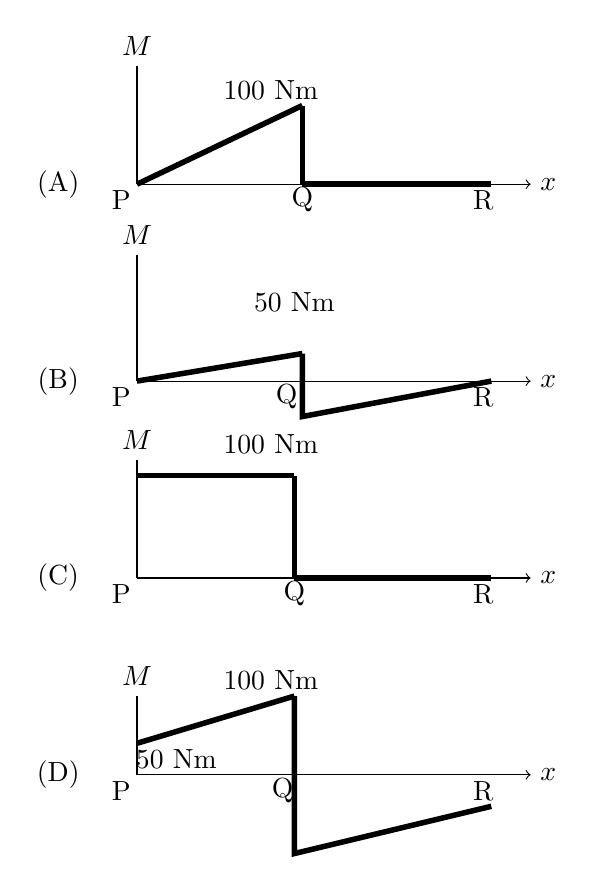
\begin{tikzpicture}

% Diagram (A)
\node at (-2.5,3.5) {(A)};
\draw[->] (-1.5,3.5) -- (3.5,3.5) node[anchor=west] {$x$};
\draw[thick] (-1.5,3.5) -- (-1.5,5) node[above] {$M$}; % M label at the top
\draw[line width=0.7mm] (-1.5,3.5) -- (0.6,4.5); % increasing slope from P to Q
\draw[line width=0.7mm] (0.6,4.5) -- (0.6,3.5);
\draw[line width=0.7mm] (0.6,3.5) -- (3,3.5); % horizontal line from Q to R
\node at (0.2,4.7) {100 Nm};
\node at (-1.7,3.3) {P};
\node at (0.6,3.3) {Q};
\node at (2.9,3.3) {R};

% Diagram (B)
\node at (-2.5,1) {(B)};
\draw[->] (-1.5,1) -- (3.5,1) node[anchor=west] {$x$};
\draw[thick] (-1.5,1) -- (-1.5,2.6) node[above] {$M$}; % M label at the top
\draw[line width=0.7mm] (-1.5,1) -- (0.6,1.35); % increasing slope from P to Q
\draw[line width=0.7mm] (0.6,1.35) -- (0.6,0.55) -- (3,1); % line with a slope from Q to R
\node at (0.5,2) {50 Nm};
\node at (-1.7,0.8) {P};
\node at (0.4,0.8) {Q};
\node at (2.9,0.8) {R};

% Diagram (C)
\node at (-2.5,-1.5) {(C)};
\draw[->] (-1.5,-1.5) -- (3.5,-1.5) node[anchor=west] {$x$};
\draw[thick] (-1.5,-1.5) -- (-1.5,0) node[above] {$M$}; % M label at the top
\draw[line width=0.7mm] (-1.5,-0.2) -- (0.5,-0.2); % constant from P to Q
\draw[line width=0.7mm] (0.5,-0.2) -- (0.5,-1.5);
\draw[line width=0.7mm] (0.5,-1.5) -- (3,-1.5); % horizontal line from Q to R
\node at (0.2,0.2) {100 Nm};
\node at (-1.7,-1.7) {P};
\node at (0.5,-1.7) {Q};
\node at (2.9,-1.7) {R};

% Diagram (D)
\node at (-2.5,-4) {(D)};
\draw[->] (-1.5,-4) -- (3.5,-4) node[anchor=west] {$x$};
\draw[thick] (-1.5,-4) -- (-1.5,-3) node[above] {$M$}; % M label at the top
\draw[line width=0.7mm] (-1.5,-3.6) -- (0.5,-3); % increasing slope from P to Q
\draw[line width=0.7mm] (0.5,-3) -- (0.5,-5) -- (3,-4.4); % line with a slope from Q to R
\node at (0.2,-2.8) {100 Nm};
\node at (-1,-3.8) {50 Nm};
\node at (-1.7,-4.2) {P};
\node at (0.35,-4.2) {Q};
\node at (2.9,-4.2) {R};

\end{tikzpicture}


